% ============================================================================
% Lignes de niveau de M -> MA^2 + MB^2 : cercles de centre I
% Extrait de la fiche : Barycentres et lignes de niveau (classe de 1ere D)
% Necessite \usepackage{tikz} et \usetikzlibrary{calc} (charges par le fichier principal)
% ============================================================================
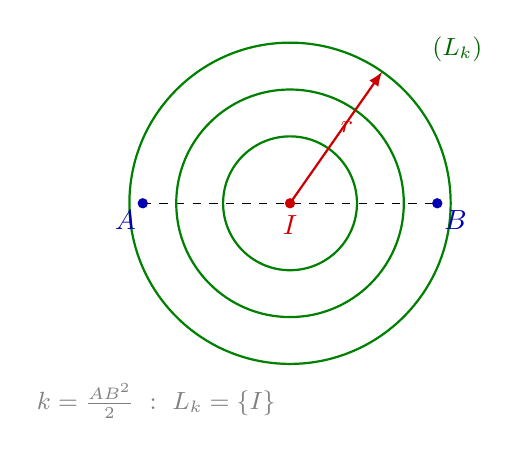
\begin{tikzpicture}[scale=0.85,>=latex]
  \coordinate (A) at (-2.2,0); \coordinate (B) at (2.2,0);
  \draw[dashed] (A) -- (B);
  \foreach \r in {1.0,1.7,2.4} {\draw[thick,green!50!black] (0,0) circle (\r);}
  \draw[->,red!80!black,thick] (0,0) -- (55:2.4) node[midway,above right=-2pt,font=\small] {$r$};
  \fill[blue!70!black] (A) circle (2.2pt) node[below left=-1pt] {$A$};
  \fill[blue!70!black] (B) circle (2.2pt) node[below right=-1pt] {$B$};
  \fill[red!80!black] (0,0) circle (2.2pt) node[below=1pt] {$I$};
  \node[green!40!black,font=\small] at (2.5,2.3) {$(L_k)$};
  \node[font=\small,gray] at (-2.0,-2.95) {$k=\frac{AB^2}{2}\ :\ L_k=\{I\}$};
\end{tikzpicture}
